\section{Results and Analysis}

\subsection{Experimental Setup}

We evaluate the proposed feature based RUL prediction pipeline on the XJTU-SY bearing dataset using the cross condition protocol described in Section~\ref{sec:evaluation_protocol}. 
The main experiment uses wavelet domain features and a sequence length of $K=40$ for neural sequence models. 
Ridge regression uses the current feature vector only and therefore does not require a sequence length. 
All feature scaling, feature screening, hyperparameter selection, and early stopping decisions are made using only the training and validation trajectories. 
The test condition is used only once for final evaluation.

We compare Ridge regression, LSTM, TCN, Transformer, and Latent ODE. 
For Ridge regression, the regularization strength is selected using validation MAE. 
For neural models, we train with Adam and select the checkpoint with the best validation error. 
The neural hyperparameters, including hidden dimension, dropout rate, learning rate, and model depth, are selected using validation trajectories only. 
We report MAE, RMSE, and Spearman correlation. 
All metrics are first computed for each test bearing and then averaged across bearings and held out operating conditions.

\subsection{Feature Setting Ablation}

We first examine how different feature settings affect cross condition prediction. 
This experiment uses Ridge regression so that the effect of the feature representation can be studied without the additional complexity of a sequence model. 
Figure~\ref{fig:feature_ablation} compares time domain features, frequency domain features, wavelet domain features, the original time and frequency feature set, the fully expanded feature set, and compact top-$k$ subsets selected from the expanded feature space.

\begin{figure}[t]
    \centering
    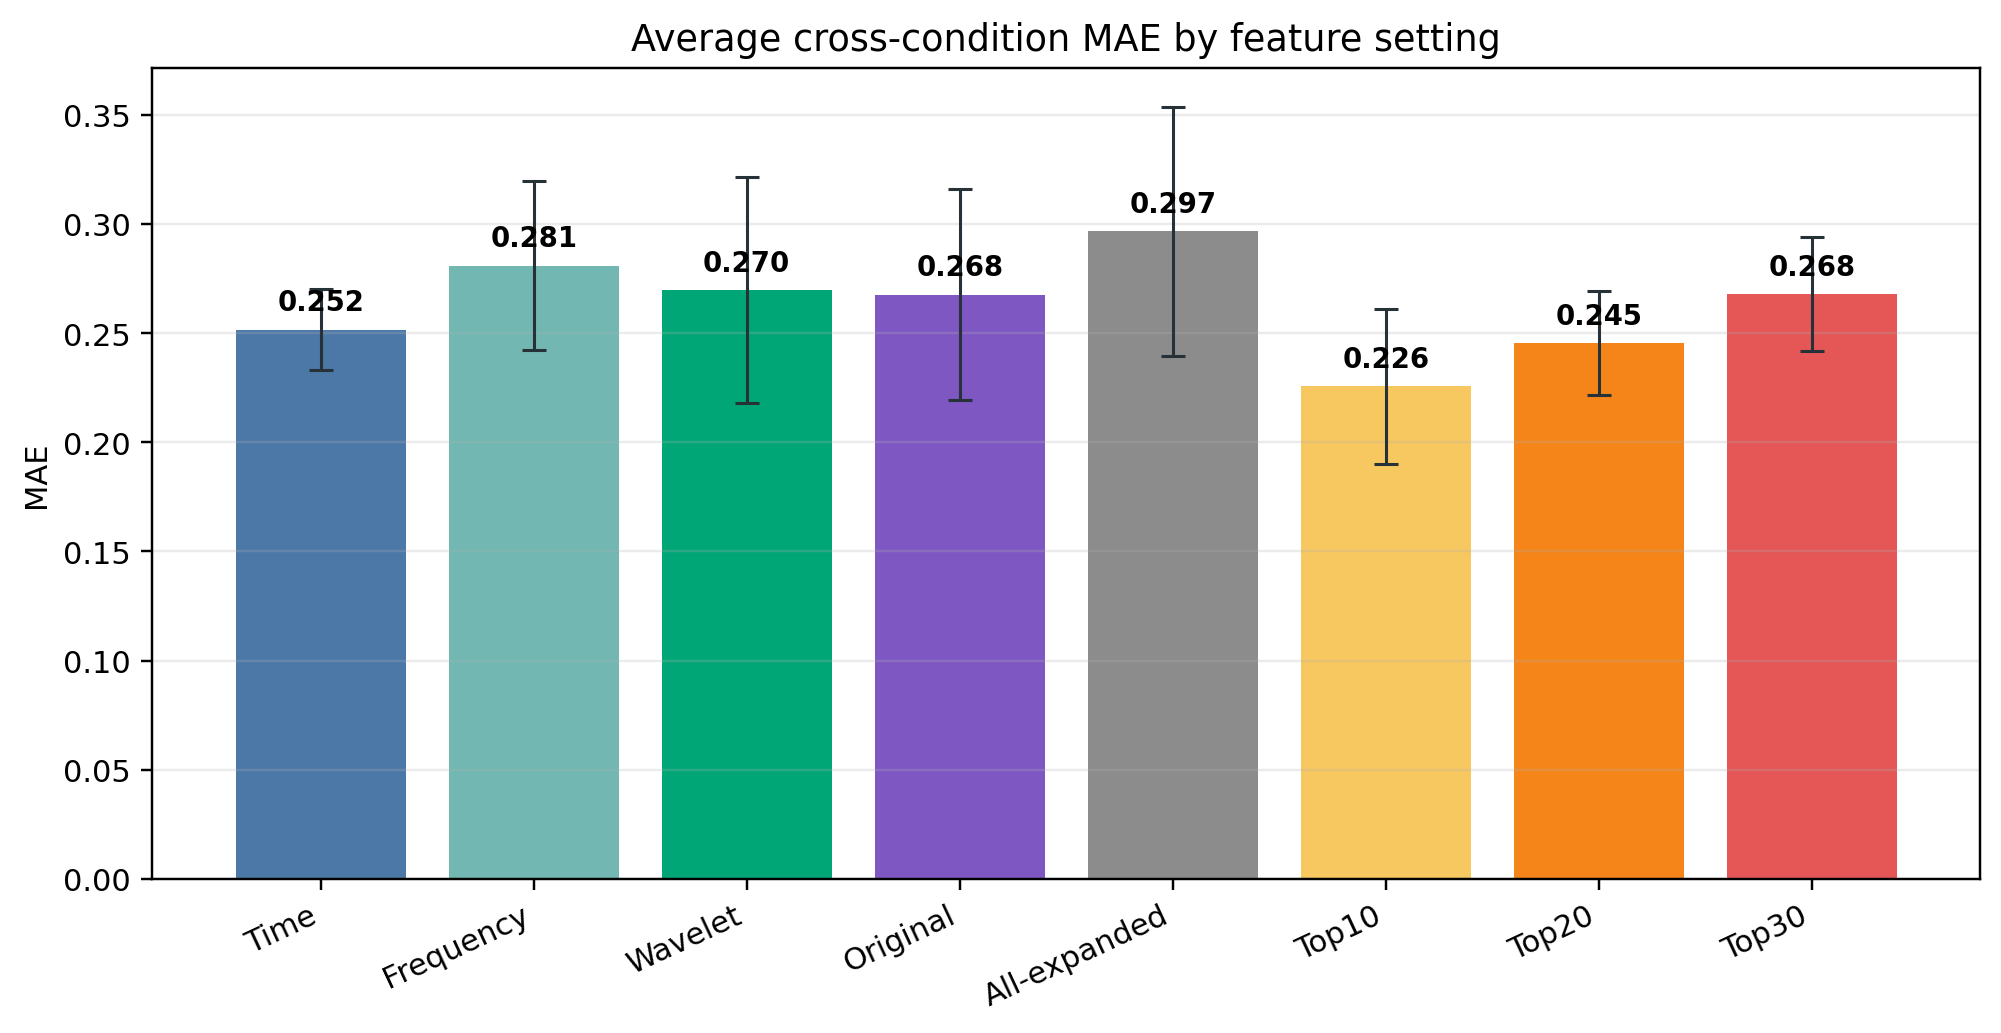
\includegraphics[width=0.70\textwidth]{figures/ridge_feature_ablation_bar.png}
    \caption{
    Feature setting ablation using Ridge regression under the cross condition protocol. 
    Lower MAE is better. 
    Compact train only feature screening reduces redundancy in the expanded feature space.
    }
    \label{fig:feature_ablation}
\end{figure}

The compact selected feature sets perform better than directly using the full expanded feature set. 
In particular, selected top 10 features achieve the lowest Ridge MAE among the compared feature settings. 
This suggests that simply concatenating all available features is not always beneficial, because the expanded feature space can introduce redundant or condition specific components. 
The ablation therefore motivates the use of controlled feature settings and train only feature screening.

\subsection{Sequence Length Selection}

For neural sequence models, the temporal window length $K$ controls how much historical information is provided to the model. 
A larger $K$ gives the model a longer degradation history, but it also removes short bearing trajectories that cannot form complete windows. 
We therefore select $K$ using validation performance together with trajectory coverage.

\begin{figure}[t]
    \centering
    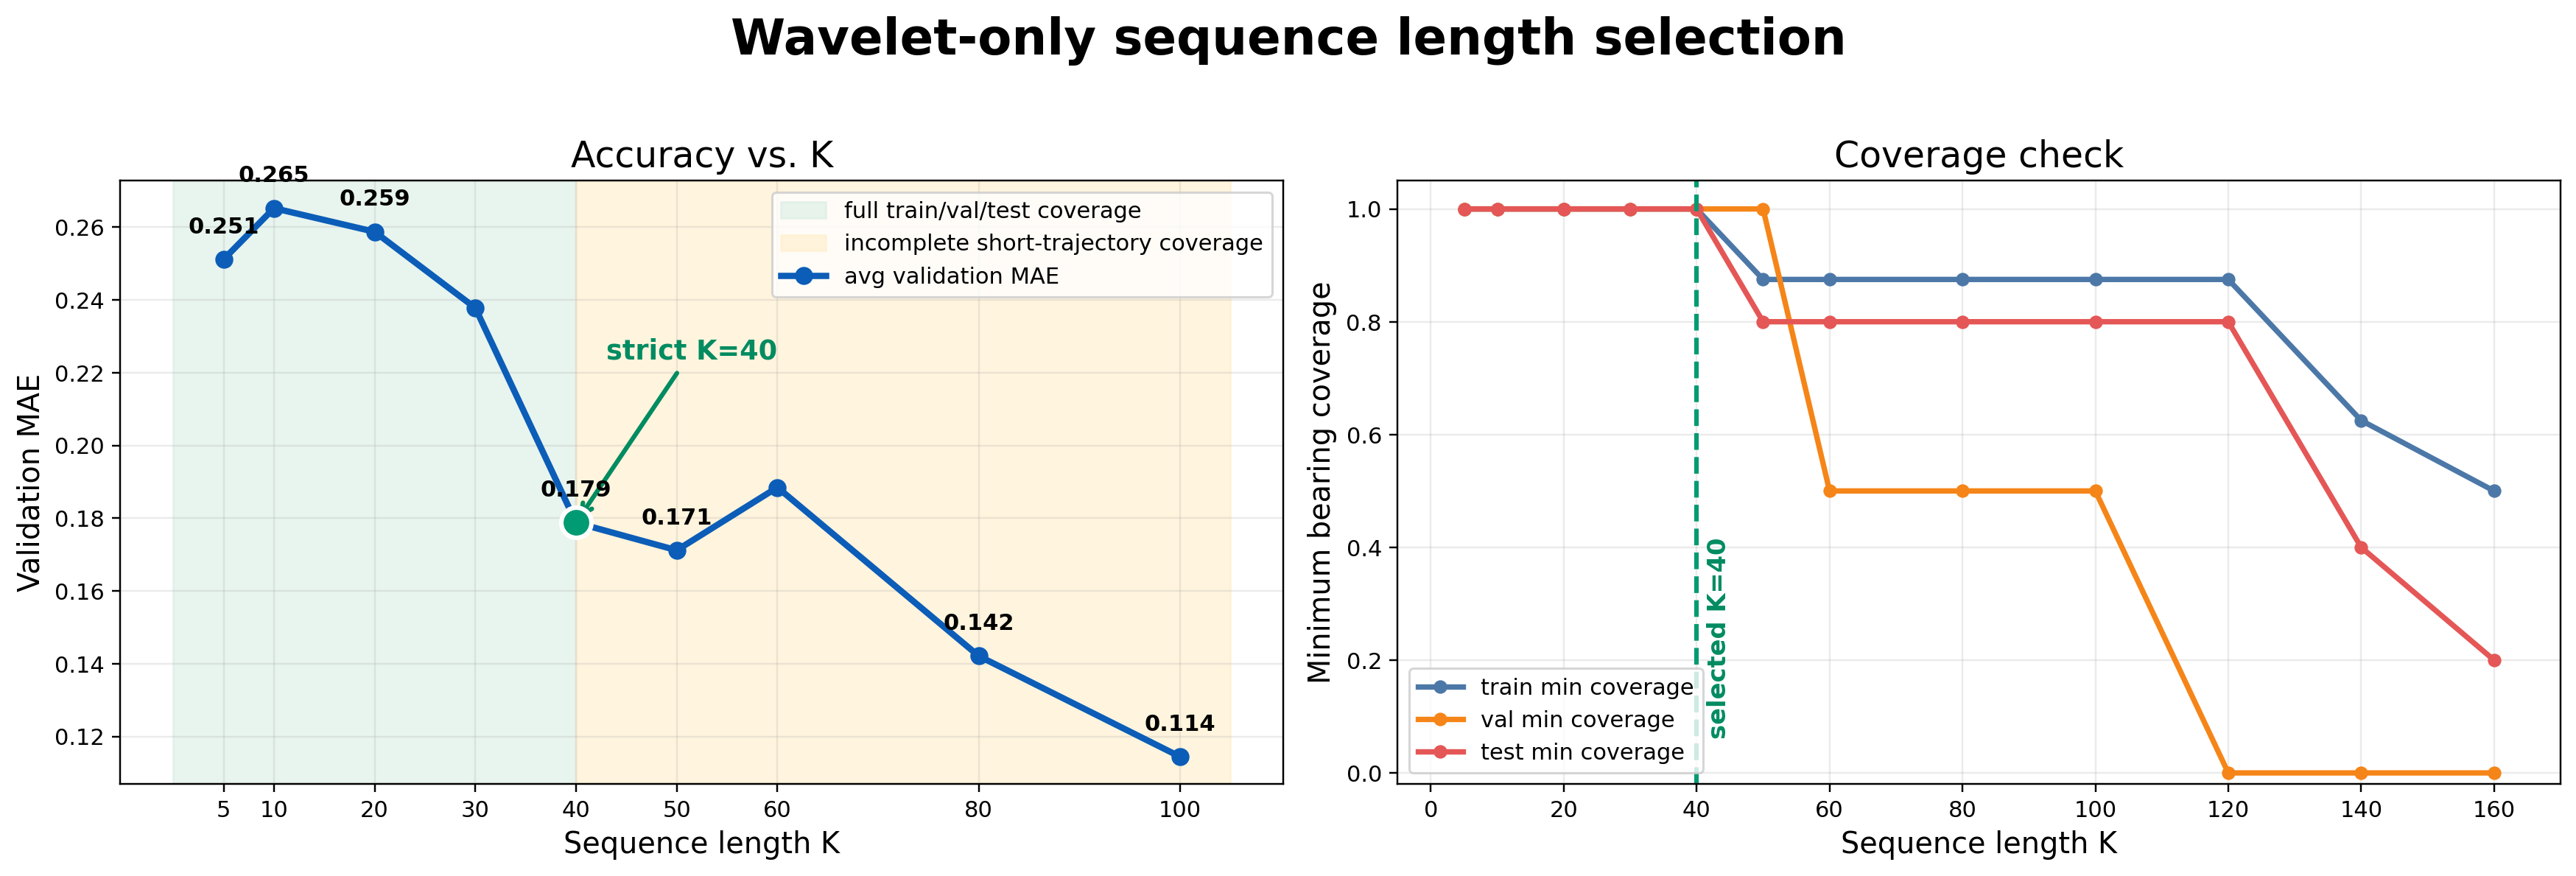
\includegraphics[width=0.78\textwidth]{figures/k_selection_v2_accuracy_coverage.png}
    \caption{
    Sequence length selection for wavelet based sequence models. 
    Longer windows can improve validation error, but overly long windows reduce the number of usable trajectories. 
    We use $K=40$ for the main experiment because it preserves full train, validation, and test coverage while maintaining competitive validation error.
    }
    \label{fig:k_selection}
\end{figure}

The raw lowest validation MAE occurs at a larger window length, but this setting removes some short trajectories. 
Since the goal of this work is a strict and comparable cross condition evaluation, we choose $K=40$ as the main setting. 
This choice preserves full coverage across training, validation, and test trajectories, while still allowing sequence models to use sufficient degradation history.

\subsection{Main Cross Condition Results}

Table~\ref{tab:main_cross_results} reports the main cross condition results after validation based model selection. 
All models are evaluated on operating conditions that are not used during training or validation. 
The TCN achieves the lowest MAE and RMSE, indicating the best point prediction accuracy in this setting. 
Transformer and LSTM obtain higher Spearman correlation than TCN, suggesting stronger ranking consistency over the bearing lifetime. 
All neural sequence models except Latent ODE outperform the classical Ridge baseline in MAE.

\begin{table}[t]
    \centering
    \caption{
    Main cross condition results using wavelet features and $K=40$ for neural sequence models. 
    Values are reported as mean $\pm$ standard deviation across the three held out operating conditions. 
    Lower MAE and RMSE are better, while higher Spearman correlation is better.
    }
    \label{tab:main_cross_results}
    \begin{tabular}{lccc}
        \hline
        Model & MAE & RMSE & Spearman \\
        \hline
        TCN & $\mathbf{0.167 \pm 0.060}$ & $\mathbf{0.202 \pm 0.069}$ & $0.508 \pm 0.054$ \\
        Transformer & $0.187 \pm 0.030$ & $0.225 \pm 0.038$ & $\mathbf{0.547 \pm 0.144}$ \\
        LSTM & $0.199 \pm 0.022$ & $0.232 \pm 0.028$ & $0.544 \pm 0.033$ \\
        Ridge & $0.252 \pm 0.033$ & $0.300 \pm 0.037$ & $0.444 \pm 0.121$ \\
        Latent ODE & $0.266 \pm 0.025$ & $0.307 \pm 0.026$ & $0.165 \pm 0.066$ \\
        \hline
    \end{tabular}
\end{table}

\begin{figure}[t]
    \centering
    \begin{minipage}{0.46\textwidth}
        \centering
        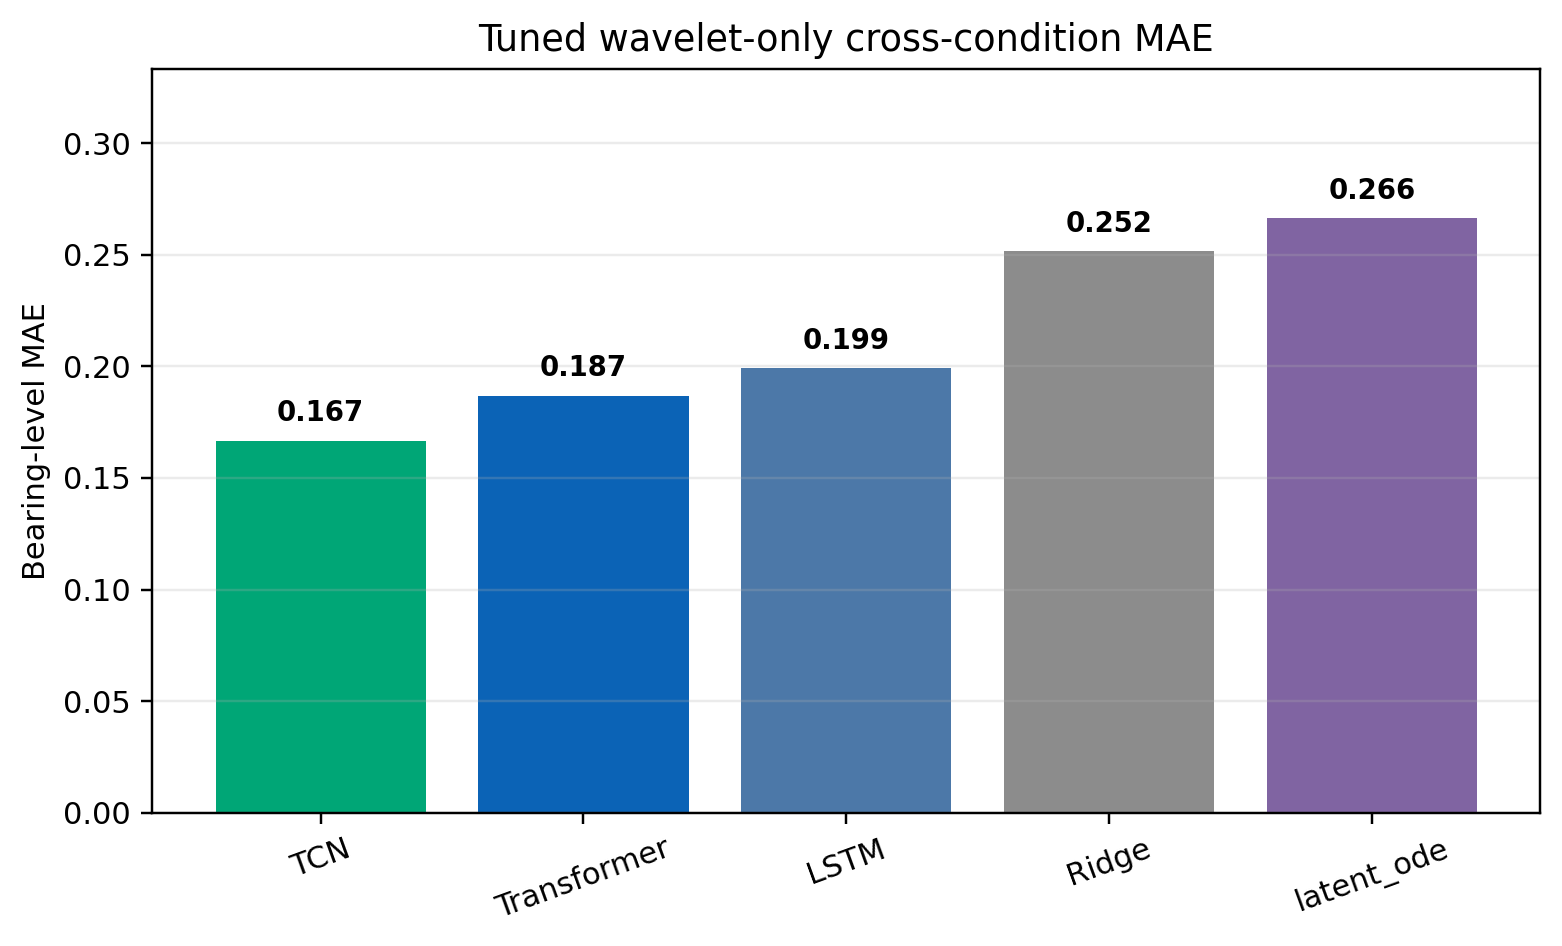
\includegraphics[width=\textwidth]{figures/tuned_wavelet_k40_cross_mae_bar.png}
    \end{minipage}
    \hfill
    \begin{minipage}{0.50\textwidth}
        \centering
        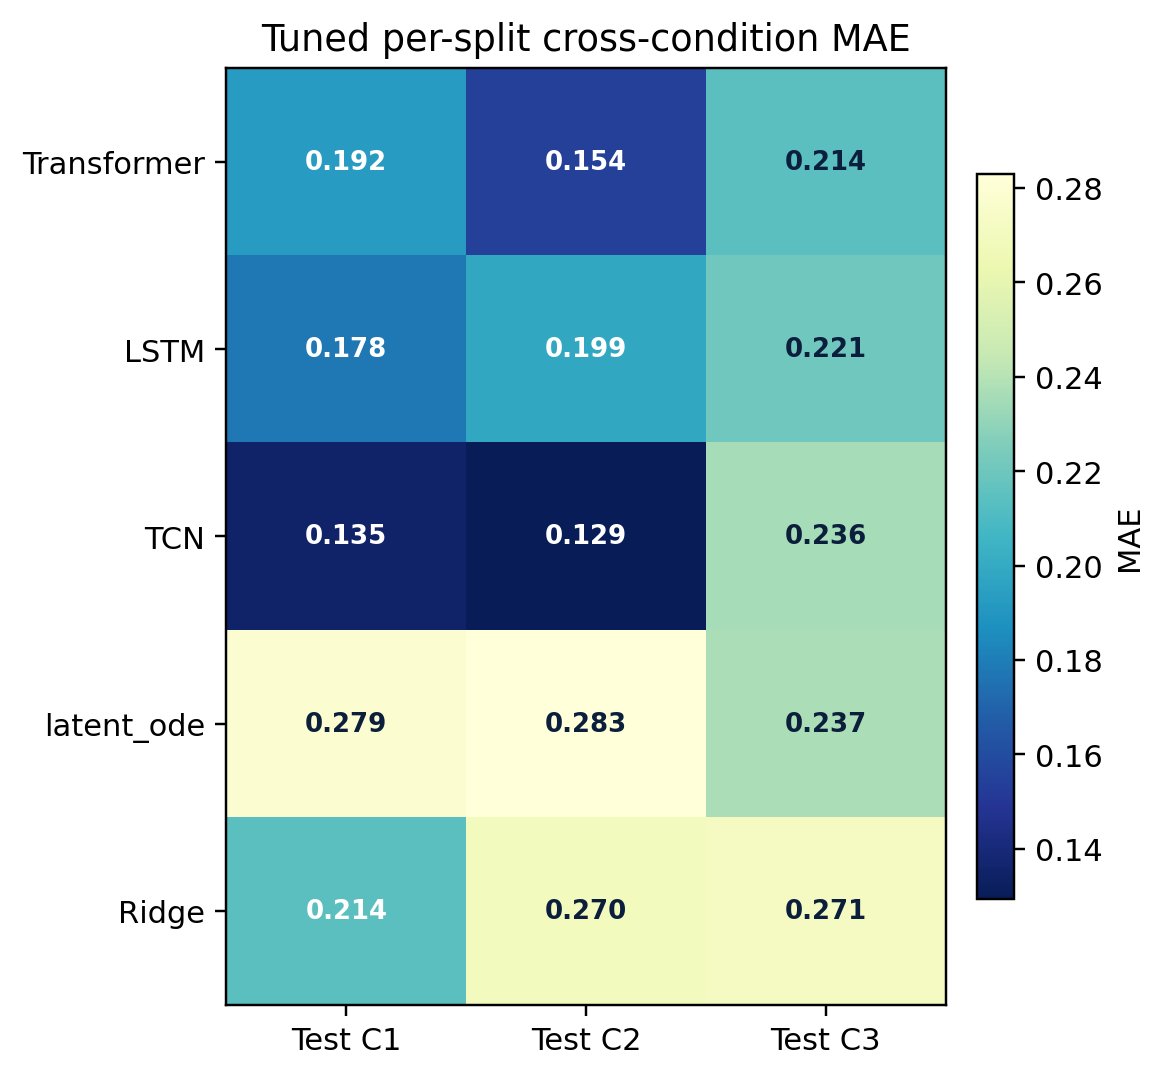
\includegraphics[width=\textwidth]{figures/tuned_wavelet_k40_per_split_heatmap.png}
    \end{minipage}
    \caption{
    Cross condition prediction results. 
    Left: average MAE across held out operating conditions. 
    Right: per split MAE, where each column corresponds to one held out test condition.
    }
    \label{fig:main_cross_results}
\end{figure}

Figure~\ref{fig:main_cross_results} further shows the per split behavior. 
The held out C3 condition is generally more difficult for the tuned sequence models than C1 and C2. 
This supports the motivation for cross condition evaluation: performance depends strongly on the operating condition used for testing, and random window level splits would not reveal this difficulty.

\subsection{Analysis}

The results lead to three main observations. 
First, operating condition shift is a major challenge for bearing RUL prediction. 
Even though all models are trained on run to failure trajectories, the held out condition can produce different degradation patterns, which increases prediction error. 
Second, temporal modeling improves cross condition prediction. 
The best sequence models outperform Ridge, showing that using a history of vibration features is more informative than using only the current time step. 
Third, model complexity must be controlled carefully. 
The TCN provides the best overall point accuracy, while Transformer and LSTM provide stronger trend consistency according to Spearman correlation. 
Latent ODE performs worse in this setting, suggesting that the available trajectory level data may not be sufficient for more complex continuous time dynamics.

Figure~\ref{fig:representative_trajectory} provides a qualitative example on the unseen C3 condition. 
The predicted trajectories generally decrease as the bearing approaches the end of the recorded run, but different models show different levels of smoothness and bias. 
This figure is used only as a qualitative check; the main conclusions are based on the bearing level metrics in Table~\ref{tab:main_cross_results}.

\begin{figure}[t]
    \centering
    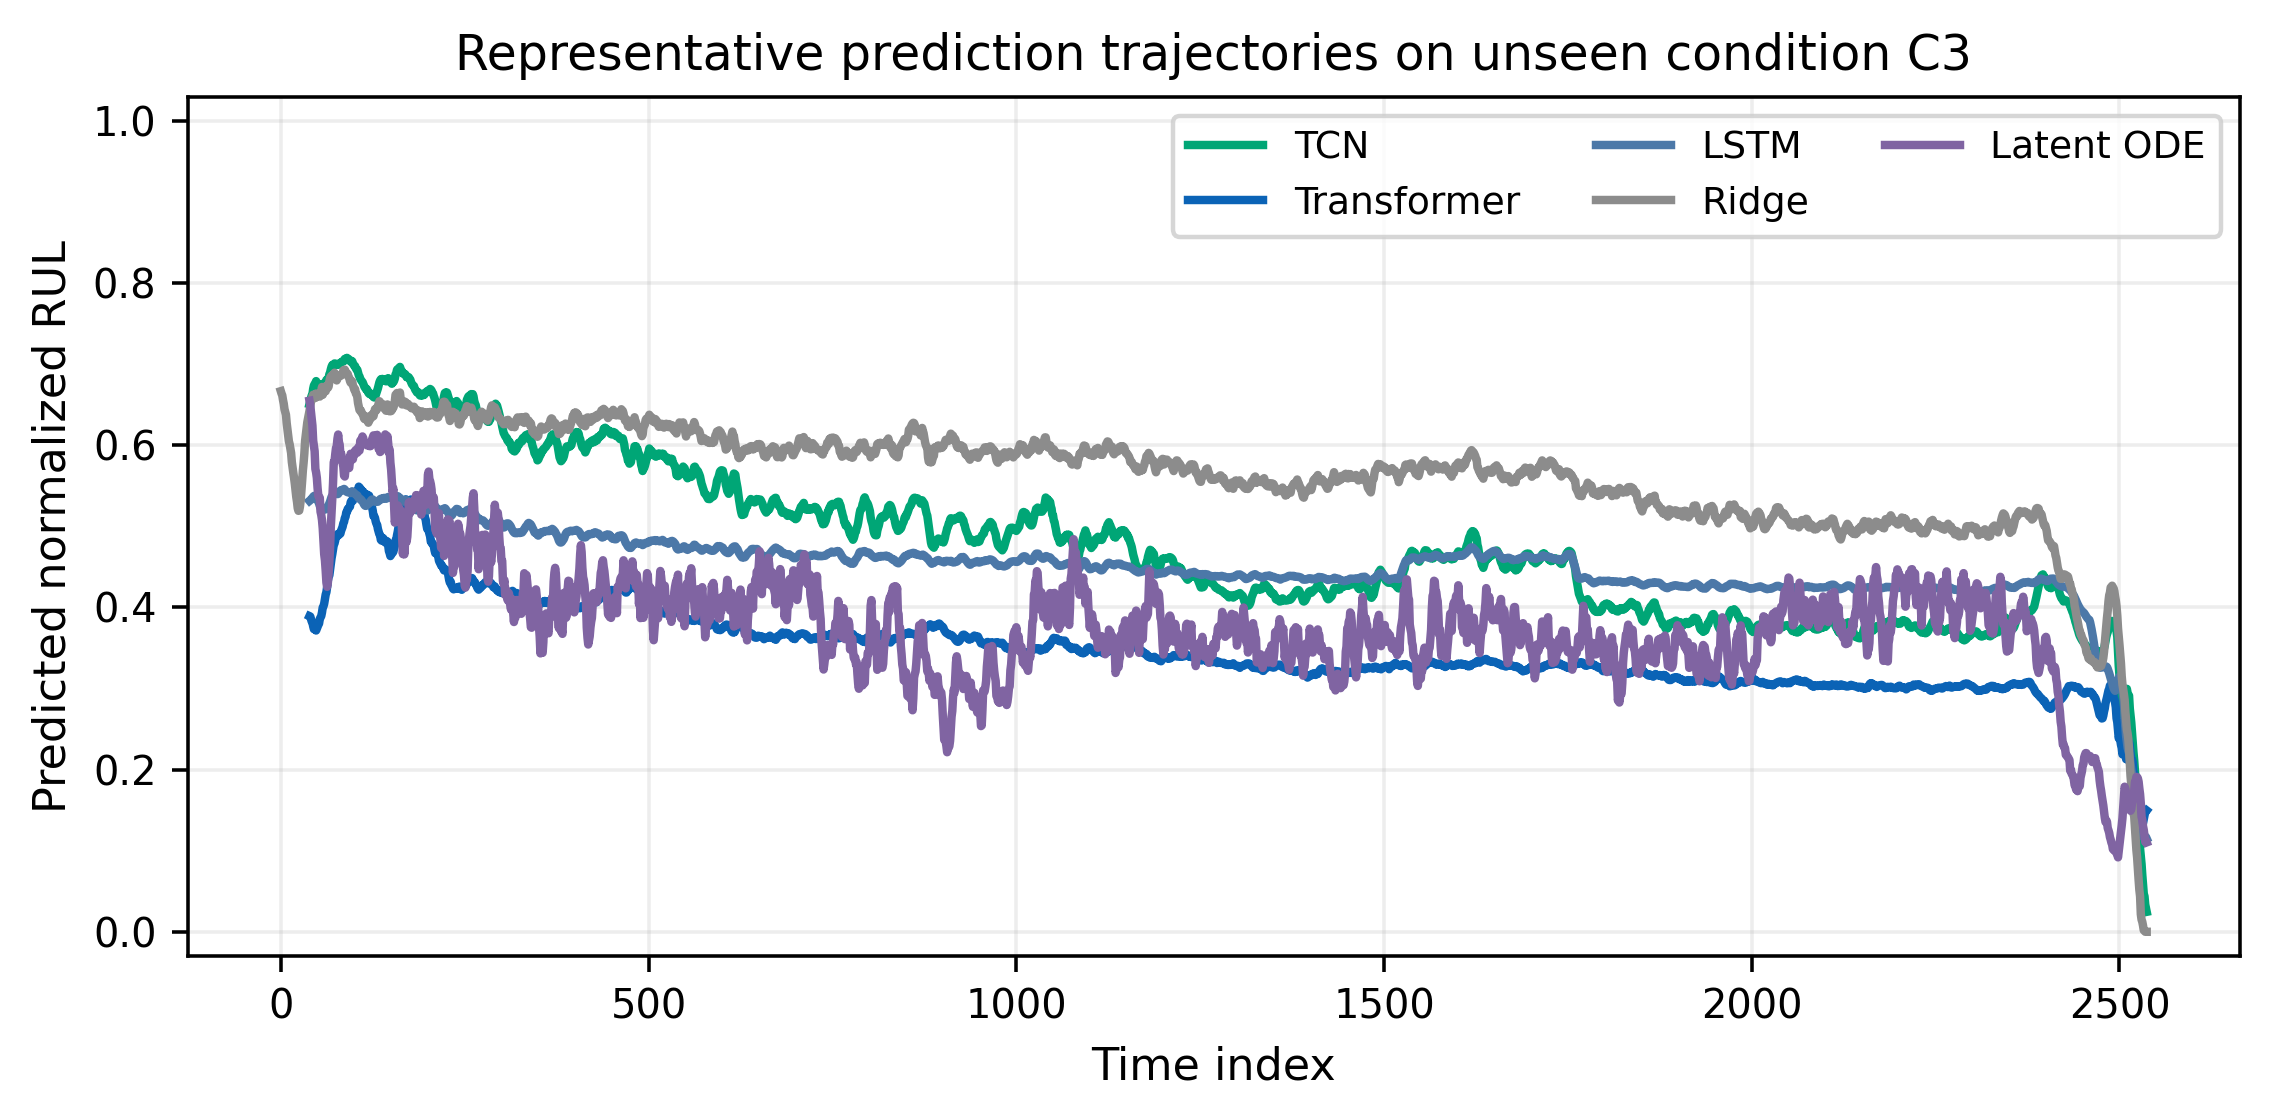
\includegraphics[width=0.78\textwidth]{figures/tuned_representative_prediction_trajectory_no_target.png}
    \caption{
    Representative prediction trajectories on an unseen C3 bearing. 
    The curves show predicted normalized RUL from models trained without access to C3 trajectories.
    }
    \label{fig:representative_trajectory}
\end{figure}

